\documentclass[12pt,titlepage]{article}





%PACKAGES
\usepackage[ngerman]{babel}
\usepackage[utf8]{inputenc}
\usepackage[a4paper,lmargin={2.5cm},rmargin={2.5cm},
tmargin={2.5cm},bmargin = {2.5cm}]{geometry}
\usepackage{graphicx}
\usepackage{caption}
\usepackage{float}
\usepackage{hyperref}
\usepackage{graphicx,wrapfig,lipsum}
\usepackage{wasysym}
\parindent0pt



\begin{document}



\thispagestyle{empty}

%TITELSEITE
\begin{center}
\textbf{Hochschule Luzern}\\
Departement für Informatik\\[12\baselineskip]

\begin{Huge}
PCP Projekt - Programmiersprachanalyse
\end{Huge} \\[6\baselineskip]

\begin{large}
\textbf{Analyse der Programmiersprache GO}
\end{large} \\[6\baselineskip]

\begin{large}
\textbf{Studierende}: Frederico Fischer, Oliver Werlen\\
\textbf{Dozenten}: Prof. Dr. Ruedi Arnold, Marcel Baumann \\

\textbf{Abgabedatum}: 26. Mai 2021 \\
\end{large}
\end{center}
\newpage


\section{Einleitung}
In dieser Projektarbeit wurde die Programmiersprache \textbf{Go} analysiert.
Es handelt es sich, wie auch bei vielen anderen Sprachen, um eine Multiparadigmensprache (funktional, imperativ und objektorientiert).
Dabei wurde Bezug auf dessen Entstehungsgeschichte sowie Spezialitäten und Feinheiten genommen.
Motivierungsgründe für die Wahl dieser Sprache waren, dass es sich dabei um eine sehr junge und oft verwendete Sprache handelt, die bei vielen neuen Anwendungen genutzt wird und eine hohe Popularität aufweist.

\section{Vision, Geschichte \& Verbreitung}
Die Sprache \glqq Go\grqq{} ist durch Google von den Entwicklern Robert Griesemer, Rob Pike und Ken Thompson entstanden.
Gründe für dessen Entstehung waren die Beseitigung der Langsam- sowie Schwerfälligkeiten und die Erhöhung der Produktivität und Skalierbarkeit ihrer Prozesse.
Das Zielpublikum dieser Sprache sind insbesondere Software Entwickler, welche sich mit grossen Softwaresystemen auseinandersetzen.
Diese Sprache zeichnet sich durch seine Performance, Lesbarkeit, unkomplizierte Einbindung von Abhängigkeiten sowie simple Nebenläufigkeitsimplementierung aus.
Insbesondere in der DevOps-Gemeinde wurde diese sehr beliebt.
Beispielsweise wurde Kubernetes in dieser Sprache entwickelt

\section{Sprachkonstrukte}
\subsection{Goroutines, Channels \& Select}
\paragraph{Goroutines}
\begin{wrapfigure}{r}{5.5cm}
	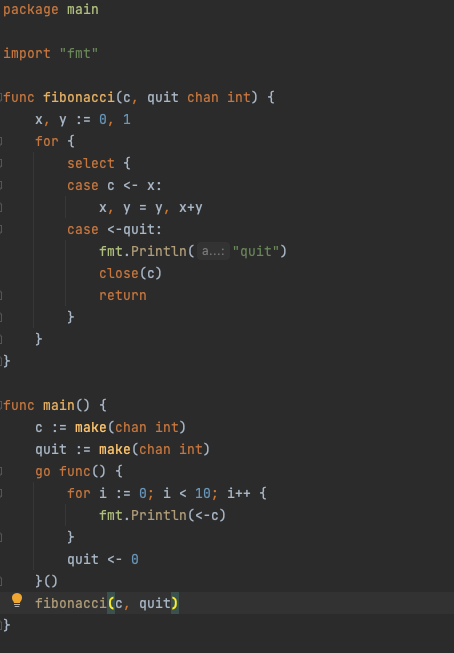
\includegraphics[width=5.5cm]{fibGoroutine}
	\caption{Beispiel Goroutine, Channel und Select}\label{img: fibGoroutine}
\end{wrapfigure}
Eine Goroutine ist ein leichtgewichtiger Thread, welcher von der Go runtime gemanaged wird.
Goroutines nutzen dabei den selben Adressraum, daher muss der Zugriff auf geteilte Ressourcen synchronisiert werden.
In Go gibt es Primitives, welche die Synchronisierung übernehmen. Jedoch werden diese nur selten genutzt, da in den meisten Fällen mit Channels gearbeitet wird.
\paragraph{Channels}
Ein Channel erlaubt einen einfachen Datenfluss. Per Default ist dabei das Senden und Empfangen blockierend, bis die andere Seite bereit ist. Goroutines lassen sich somit sehr leicht synchronisieren, ohne den Einsatz von Locks oder Variablen. Der Channel kann explizit vom Sender geschlossen werden. Damit wird dem Empfänger signalisiert, dass keine Werte mehr empfangen werden können. Das Schliessen des Channels sollte dabei exklusiv vom Sender ausgeführt werden. Senden auf einen geschlossenen Channel verursacht dabei "panic".
\paragraph{Select}
Bei einem Select wird bei mehrfacher Auswahl gewartet, bis eine Operation laufen kann. 

\paragraph{Beispiel}
In der Abbildung \ref{img: fibGoroutine} werden alle oben genannten Sprachkonstrukte genutzt. Bei func() handelt es sich um eine Goroutine, welche 10 Werte von dem Channel c liesst und anschliessend einen Wert auf den Quit-Channel schreibt. Das Select diffenziert dabei zwischen den beiden Channels. Je nach Case wird entweder eine neue Fibonacci-Zahl berechnet oder der Channel geschlossen.

\begin{wrapfigure}{r}{0.5\linewidth}
	\centering
	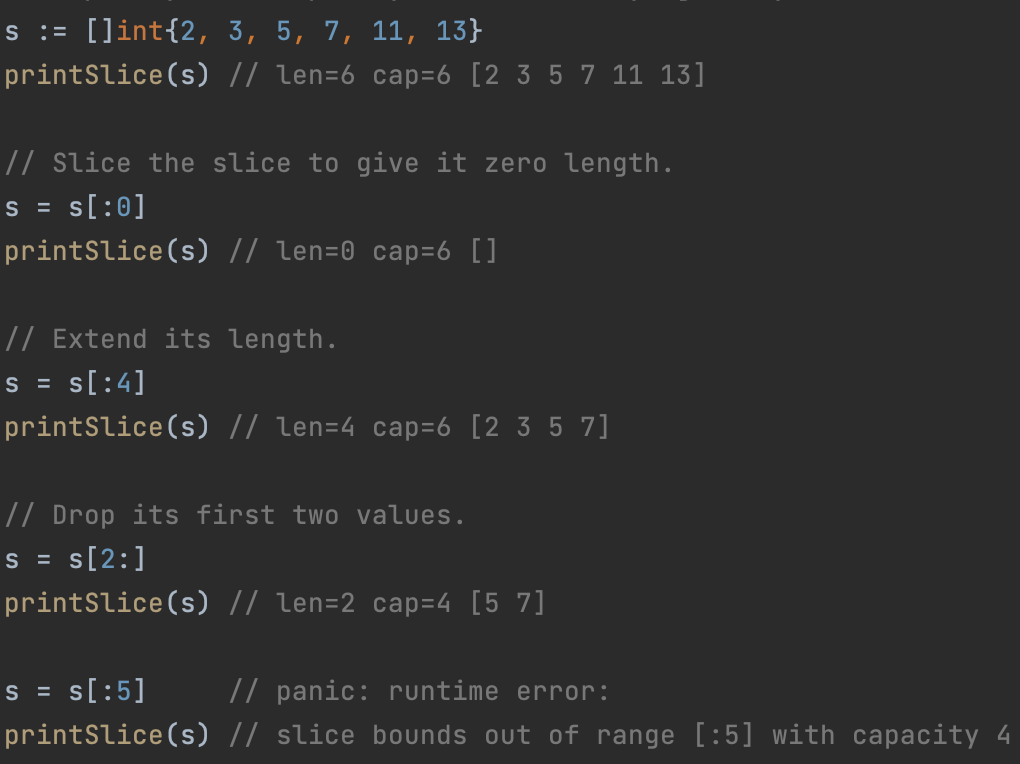
\includegraphics[width=7.5cm]{slices}
	\caption{Verhalten von Slices, Quelle Autor}\label{slices}
\end{wrapfigure}
\subsection{Maps \& Slices}
\paragraph{Slices}
Bei Slices handelt es sich um ein dynamisches Array welches speziell für Go implementiert wurde und als Datenstruktur in der Standardbibliothek mitenthanlten ist.
Im Untergrund besteht ein Slice aus einem Array weshalb es auch Funktionen eines Arrays mitliefert.
Ein wichtiger Unterschied ist, dass ein Array ein Value-Typ ist, wohingegen ein Slice ein Referenz-Typ.
Bei der Instanzierung eines Slices kann dessen Länge sowie Kapazität angegeben werden.
Die Länge bezeichnet die Anzahl Elemente welches ein Slice enthält und die Kapazität die Anzahl Elemente welche sich im unterliegenden Array befinden.

\paragraph{Maps}
\begin{wrapfigure}{l}{0.5\linewidth}
	\centering
	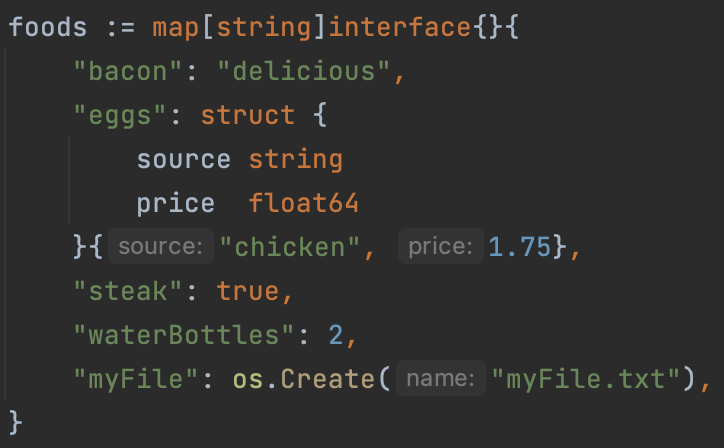
\includegraphics[width=8cm]{map-example}
	\caption{Beispiel einer Map, Quelle Autor}\label{map}
\end{wrapfigure}
Hierbei handelt es sich um eine Key-Value-Datenstruktur, welche in anderen Sprache unter HashMaps bekannt ist.
Typen von Keys müssen comparable sein, weshalb Funktionen und Slices nicht genommen werden können.
Eine spezielle Eigenschaft dieser Map ist der Value-Type \textbf{Interface}.
Damit steht als Value dem Entwickler offen was für Typen dieser dort nutzen will.
Es kann eine Mischung aus Structs, Strings, Arrays, Pointers etc. sein.
Diese Eigenschaft ist nützlich, wenn bspw. das Schema vom erhaltenen JSON nicht bekannt ist und in einer Map gespeichert werden soll.
map interface!

\subsection{Structural \& Nominal Typing}
Erklärung und Codebeispiel


\subsection{The Go Memory Model}
\begin{wrapfigure}{l}{0.4\linewidth}
	\centering
	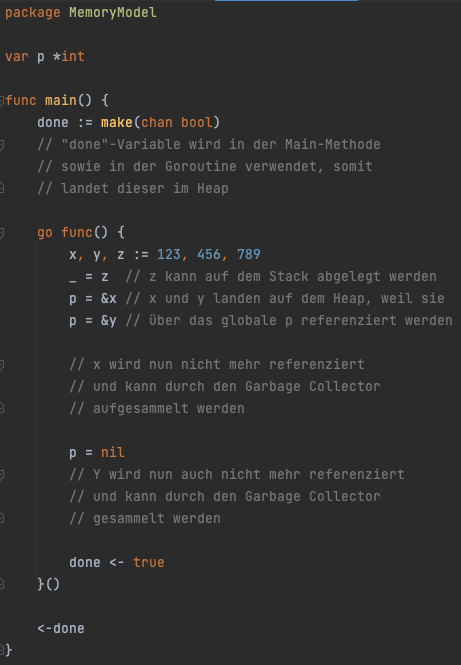
\includegraphics[width=6cm]{memorymodel}
	\caption{Beispiel vom Memory Management, Quelle Autor}\label{memorymodel}
\end{wrapfigure}
Die Sprache \textbf{Go} liefert ein automatisches Memory Management mit wie zum Beispiel automatische Memoryallozierung oder den Garbage Collector.
Dieser arbeitet dabei mit Memory Blocks, welche Values beinhalten und unterschiedlich gross sein können.
Memory Blocks entstehen bspw. durch den Aufruf von \textbf{new} (nur einen auf dem Heap oder Stack) oder \textbf{make} (mehrere auf dem Heap), Variablendeklarationen etc.
Jede goroutine verwaltet einen Stack (Memory Segment).
Dabei handelt es sich um einen Memory Pool von Memory Blocks welche alloziert werden können.
Memory Blocks, welche durch eine Goroutine auf einen Stack alloziert werden, sind nur in dieser Goroutine intern ersichtlich.
Darin müssen keine Synchronisationsarbeiten vorgenommen werden.
Beim Heap handelt es sich um ein Singleton.
Wenn ein Memory Block nicht in einer Goroutine Stack alloziert ist, landet er im Heap.
Solche Memory Blöcke können durch mehrere Goroutine verwendet werden, weshalb die Synchronisierung beachtet werden muss.
Wenn der Compiler entdeckt, dass ein Memory Block über mehrere Goroutines hinweg verwendet wird oder sich nicht sicher ist ob es auf den Stack soll, wird dieser im Heap abgelegt.
Die Vorteile Memory Blocks auf dem Stack abzulegen sind, dass die Allozierung schneller ist, diese nicht durch den Garbage Collector bereinigt werden müssen und sie CPU Cache-freundlicher sind.

\subsection{Package Management}
Erklärung und Codebeispiel


\subsection{Defer}
Erklärung und Codebeispiel

\section{Fazit}
\subsection{Team-Fazit}

\subsection{Fazit Frederico Fischer}

\subsection{Fazit Oliver Werlen}

    

\end{document}